Per il progetto è stato sviluppato un plugin per Eclipse che si occupa di: \\*
\begin{itemize}
  \item text-highlight
  \item controllo degli errori
  \item compilazione
\end{itemize} 


\subsection{text-hilight}
Il plugin gestisce il \emph{modello dati} e lo \emph{schema di layout} in modi differenti; 
entrambi, infatti, presentano caratteristiche e strutture diverse tra loro.
La classe che esegue la scansione del \emph{modello dati} e ne gestisce l'editor
è la seguente:

\begin{lstlisting}[caption={ModelScanner}, style={java}]
public class ModelScanner extends RuleBasedScanner {
	//TODO controllare tutte le keyword
	private static String[] keywords= { "class","package", "public",
			"private","interface", "methods","extend", "relations", 
			"attributes"  };
	public ModelScanner(ColorManager manager) {
					manager.getColor(ColorConstants.DEFAULT)));
		ArrayList<IRule> rules= new ArrayList<IRule>();	
		Token tokencomment = new Token(new TextAttribute(
						manager.getColor(ColorConstants.COMMENT)));
		//Add rule for processing instructions
		rules.add( new SingleLineRule("//", "\n", tokencomment));
		rules.add( new SingleLineRule("#", "\n", tokencomment));
		rules.add( new MultiLineRule("/*", "*/", tokencomment));
		
		Token token= new Token(new TextAttribute(
				manager.getColor(ColorConstants.KEYWORD), 	//parola
				null, 	//sfondo
				SWT.BOLD));
		WordRule wordRule = new WordRule(new WordDetector());
		for (int i = 0; i < keywords.length; i++) {
			wordRule.addWord(keywords[i], token);
		}		
		rules.add(wordRule);
		
		token = new Token(new TextAttribute(
							manager.getColor(ColorConstants.BRACET)));
		RuleBrace braceRule = new RuleBrace(token);
		rules.add(braceRule);
		
		IRule[] r= new IRule[rules.size()];
		setRules(rules.toArray(r));
	}
}
\end{lstlisting}


Le parole chiave di questo modello sono specificate nella stringa
\emph{Keywords}, inoltre vengono definite le regole per i commenti e viene
utilizzata la classe RuleBrace, che è utilizzata per la gestione delle
parentesi.\\* 
La classe che esegue la scansione dello  \emph{schema di layout} e ne gestisce
l'editor, invece, è la seguente:

\begin{lstlisting}[caption={LayoutScanner}, style={java}]

public class LayoutScanner extends RuleBasedScanner {
	private static String[] keywordslayout= {"@layout","@hide-args",
												"@collapse","@margin"};
	private static String[] keywords= { "class","import","interface"};
	
	public LayoutScanner(ColorManager manager) {
		ArrayList<IRule> rules= new ArrayList<IRule>();
		Token token= new Token(new TextAttribute(
				manager.getColor(ColorConstants.KEYWORD), 	//parola
				null, 																			//sfondo
				SWT.BOLD));
		Token tokenlayout= new Token(new TextAttribute(
				manager.getColor(ColorConstants.LAYOUT), 	//parola
				null, 																		//sfondo
				SWT.BOLD));
		WordRule wordRule = new WordRule(new WordDetector());

		for (int i = 0; i < keywords.length; i++) {
			wordRule.addWord(keywords[i], token);
		}
		for (int i = 0; i < keywordslayout.length; i++) {
			wordRule.addWord(keywordslayout[i], tokenlayout);
		}
		rules.add(wordRule);
		Token tokencomment = new Token(new TextAttribute(
								manager.getColor(ColorConstants.COMMENT)));
		//Add rule for processing instructions		
		rules.add( new SingleLineRule("//", "", tokencomment));
		rules.add( new SingleLineRule("#", "", tokencomment));
		rules.add( new MultiLineRule("/*", "*/", tokencomment));
//gestione colore parentesi
		token = new Token(new TextAttribute(
										manager.getColor(ColorConstants.BRACET)));
		RuleBrace braceRule = new RuleBrace(token);
		rules.add(braceRule);
		IRule[] r= new IRule[rules.size()];
		setRules(rules.toArray(r));
	}
}



\end{lstlisting}



In questo modello le parole chiave sono specificate nella
stringa \emph{Keywords}, mentre le proprietà disponibili sono definite in
\emph{keywordslayout}, in questo modo è possibile gestirle in modo separato.
Per la gestione delle parentesi e dei commenti sono state utilizzate le stesse
tecniche del modello dello \emph{schema di layout}.

\subsection{controllo degli errori} 
Il plugins si occupa di visualizzare, tramite dei marker laterali, gli errori 
commessi in fase di scrittura del \emph{modello dati} e dello \emph{schema di
layout}. \\*
Gli errori che vengono controllati e segnalati sono:
\begin{itemize}
  \item attributo duplicato;
  \item metodo duplicato
  \item metodo con parametri con lo stesso nome
  \item dichiarazione di classe duplicata
  \item classe già inserita nella dichiarazione
  \item classe inesistente
\end{itemize} 

Il controllo degli errori viene eseguito ogni volta che il file su cui si stà lavorando
viene salvato; un esempio del funzionamento è visibile in figura \ref{errorieditor}

\begin{figure}[htp]
\begin{center}
  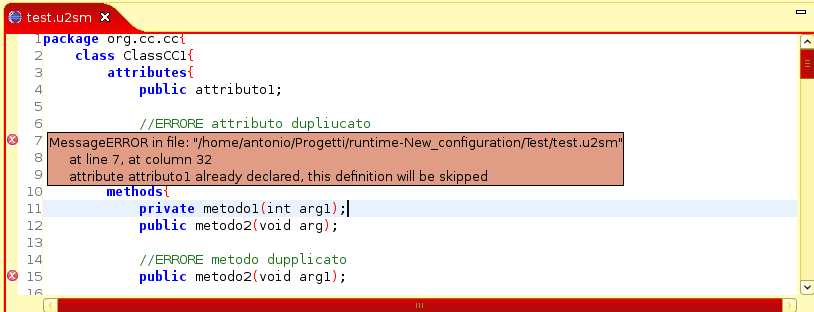
\includegraphics[width=0.9\textwidth]{img/errori_editor.png}
  \caption[labelInTOC]{Gestione degli errori}
  \label{errorieditor} 
\end{center}
\end{figure} 











\subsection{compilazione} 
Il plugins si occupa di visualizzare, tramite dei marker laterali, gli errori 
commessi in fase di scrittura del \emph{modello dati} e dello \emph{schema di
layout}. \\*
Il controllo degli errori viene eseguito ogni volta che il file su cui si stà lavorando
viene salvato; un esempio del funzionamento è visibile in figura \ref{errorieditor}
